\مسئله{}
\پاسخ{}
ابتدا تصویری از vtable مدنظر برای کلاس B ، در زیر می‌گذارم: (برای مثال آدرس methodA در خانه دوم vtable ذخیره شده است)\\
\graphicspath{{./images/}}
\begin{center}
	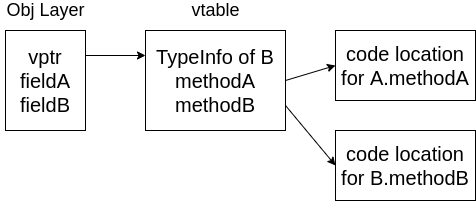
\includegraphics[scale=0.7]{Q5_1.png}
\end{center}
کد TAC در زیر نوشته شده است:
\begin{latin}
	\begin{verbatim}
		1. main:
		2. BeginFunc 24;
		3. _t0 = 16;
		4. PushParam _t0;
		5. b = LCall _Alloc;
		6. PopParams 4;
		7. _t1 = B_vtable;
		8. *b = _t1;
		9. _t2 = b + 4;
		10. *_t2 = int_default;
		11. _t3 = b + 8;
		12. *_t3 = int_default;
		13. _t0 = b + 4;
		14. *_t0 = 5;
		15. _t0 = b + 8;
		16. *_t0 = 10;
		17. _t0 = *b;
		18. _t0 = _t0 + 8;
		19. _t0 = *_t0;
		20. _t1 = 2;
		21. x = int_default;
		22. PushParam b;
		23. PushParam _t1;
		24. x = ACall _t0;
		25. PopParams 8;
		26. EndFunc;
		.
		.
		.
		27. B.methodB:
		28. BeginFunc 28;
		29. _t0 = b + 8;
		30. _t0 = *_t0;
		31. _t2 = param + _t0; 
		32. _t0 = 6;
		33. _t1 = *b;
		34. _t1 = _t1 + 4;
		35. _t1 = *_t1;
		36. PushParam b;
		37. PushParam _t0;
		38. _t3 = ACall _t1;
		39. PopParams 8;
		40. _t4 = _t3 * _t2;
		41. Return _t4;
		42. EndFunc;
		.
		.
		.
		43. A.methodA:
		44. BeginFunc 20;
		45. _t0 = b + 4;
		46. _t0 = *_t0;
		47. _t1 = a + _t0;
		48. _t2 = _t1 * 10;
		49. Return _t2;
		50. EndFunc;
	\end{verbatim}
\end{latin}
حال خطوط را به طور خلاصه توضیح می‌دهم:\\\\
در خطوط ۳ تا ۶ فضای حافظه برای object اتخاذ می‌شود.\\
در خطوط ۷ تا ۱۲ field ها و اشاره‌گر به vtable برای object مقداردهی می‌شود.\\
در خطوط ۱۳ و ۱۴ به fieldA مقدار ۵ می‌دهیم. در خطوط ۱۵ و ۱۶ هم به fieldB مقدار ۱۰ می‌دهیم.\\
در خطوط ۱۷ تا ۲۵ b.methodB را صدا می‌زنیم.\\\\
در خطوط ۲۹ تا ۳۱ مقدار param + this.fieldA بدست می‌آید.\\
در خطوط ۳۲ تا ۴۰ تابع this.methodA صدا زده می‌شود.\\
در خط ۴۱ هم مقدار تابع this.methodB برگردانده می‌شود.\\\\
در خطوط ۴۵ تا ۴۸ مقدار $(a + this.fieldA) * 10$ محاسبه می‌شود.
در خط ۴۹ هم مقدار آن برگردانده می‌شود.




